%--------------------------------------
%ELECTROTECHNIQUE - SCHEMA DE LIAISON A LA TERRE
%--------------------------------------

%utiliser les environnement \begin{comment} \end{comment} pour mettre en commentaire le préambule une fois la programmation appelée dans le document maître (!ne pas oublier de mettre en commentaire \end{document}!)

\begin{comment}

\documentclass[a4paper, 11pt, twoside, fleqn]{memoir}

\usepackage{AOCDTF}

%--------------------------------------
%CANEVAS
%--------------------------------------

\newcommand\BoxColor{\ifcase\thechapshift blue!30\or brown!30\or pink!30\or cyan!30\or green!30\or teal!30\or purple!30\or red!30\or olive!30\or orange!30\or lime!30\or gray!\or magenta!30\else yellow!30\fi} %définition de la couleur des marqueurs de chapitre

\newcounter{chapshift} %compteur de chapitre du marqueur de chapitre
\addtocounter{chapshift}{-1}
	
\newif\ifFrame %instruction conditionnelle pour les couleurs des pages
\Frametrue

\pagestyle{plain}

% the main command; the mandatory argument sets the color of the vertical box
\newcommand\ChapFrame{%
\AddEverypageHook{%
\ifFrame
\ifthenelse{\isodd{\value{page}}}
  {\backgroundsetup{contents={%
  \begin{tikzpicture}[overlay,remember picture]
  \node[
  	rounded corners=3pt,
    fill=\BoxColor,
    inner sep=0pt,
    rectangle,
    text width=1.3cm,
    text height=5.5cm,
    align=center,
    anchor=north west
  ] 
  at ($ (current page.north west) + (-0cm,-2*\thechapshift cm) $) %nombre négatif = espacement des marqueurs entre les différents chapitres (à régler en fin de rédaction) (4.5cm vaut un espacement équivalement à la hauteur du marqueur, une page peut en contenir 6 avec cet espacement-la mais il est le plus équilibré)
    {\rotatebox{90}{\hspace*{.3cm}%
      \parbox[c][0.9cm][t]{5cm}{%
        \raggedright\textcolor{black}{\sffamily\textbf{\leftmark}}}}};
  \end{tikzpicture}}}
  }
  {\backgroundsetup{contents={%
  \begin{tikzpicture}[overlay,remember picture]
  \node[
  	rounded corners=3pt,
    fill=\BoxColor,
    inner sep=0pt,
    rectangle,
    text width=1.3cm,
    text height=5.5cm,
    align=center,
    anchor=north east
  ] 
  at ($ (current page.north east) + (-0cm,-2*\thechapshift cm) $) %nombre négatif = espacement des marqueurs entre les différents chapitres (à régler en fin de rédaction) (4.5cm vaut un espacement équivalement à la hauteur du marqueur, une page peut en contenir 6 avec cet espacement-la mais il est le plus équilibré)
    {\rotatebox{90}{\hspace*{.3cm}%
      \parbox[c][0.9cm][t]{5cm}{%
        \raggedright\textcolor{black}{\sffamily\textbf{\leftmark}}}}};
  \end{tikzpicture}}}%
  }
  \BgMaterial%
  \fi%
}%
  \stepcounter{chapshift}
}

\renewcommand\chaptermark[1]{\markboth{\thechapter.~#1}{}} %redéfinition du marqueur de chapitre pour ne contenir que le titre du chapitre %à personnaliser selon le nombre de chapitre dans le cours

%--------------------------------------
%corps du document
%--------------------------------------

\begin{document} %corps du document
	\openleft %début de chapitre à gauche

\end{comment}

\begin{xltabular}{\linewidth}{p{0.3cm} m{2cm} X p{0.3cm} m{2cm} X p{0.3cm} m{2.2cm} X}
\caption{Descriptif des indices de protection} 
\\
\toprule
\multicolumn{3}{c}{\thead{Protection contre les corps solides}}	& \multicolumn{3}{c}{\thead{Lettre additionnelle\\Contact direct avec les parties dangereuses}}	& \multicolumn{3}{c}{\thead{Protection contre les liquides}} \\
\midrule
\endfirsthead %en-tête de la première page du tableau  

\toprule
\multicolumn{3}{c}{\thead{Protection contre les corps solides}}	& \multicolumn{3}{c}{\thead{Lettre additionnelle\\Contact direct avec les parties dangereuses}}	& \multicolumn{3}{c}{\thead{Protection contre les liquides}} \\
\midrule
\endhead %en-tête de la première page du tableau  

\addlinespace
\midrule %filet de milieu de tableau
\multicolumn{9}{r}{\small\textit{Page suivante}}
\endfoot %pied de page de toutes les pages du tableau

\bottomrule
\endlastfoot %pied de page de la dernièredu tableau

0 		& 									& Aucune protection	&	&	&	& 0 	&	&	Aucune protection \\
1 		& 	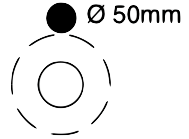
\includegraphics[scale=1.1]{1X.png} & Protégé contre les corps solides $\diameter \geq \SI{50}{\milli\meter}$  	&	A & 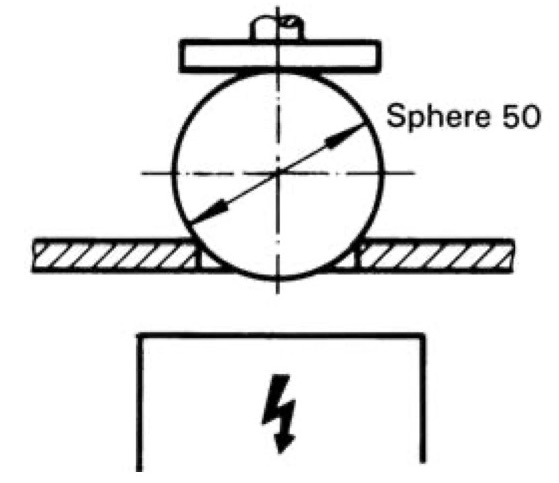
\includegraphics[width=2cm]{A.png}	&	Le dos de la main reste éloigné des parties dangereuses.	& 1 & 	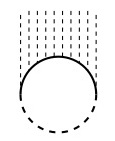
\includegraphics[scale=1.1]{X1.png}	&	Protégé contre les chutes verticales de gouttes d'eau (condensation) \\
2 		& 	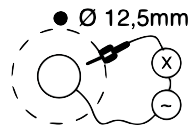
\includegraphics[scale=1.1]{2X.png} & Protégé contre les corps solides $\diameter \geq \SI{12,5}{\milli\meter}$  	& B	& 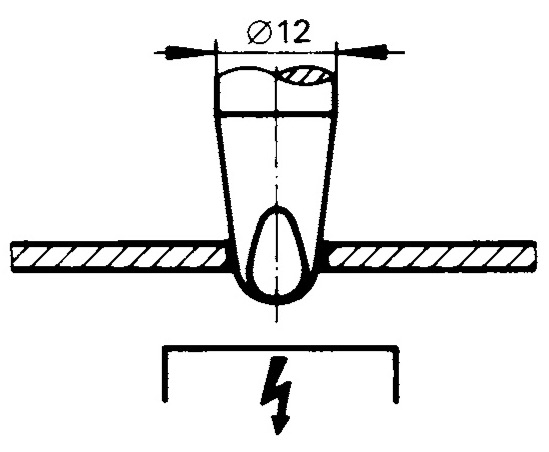
\includegraphics[width=2cm]{B.png}	&	L'introduction d'un doigt ne permet pas de toucher les parties dangereuses. & 2 & 	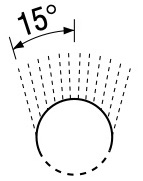
\includegraphics[scale=1.1]{X2.png}	&	Protégé contre les chutes de gouttes d'eau jusqu'à 15° de la verticale \\
3 		& 	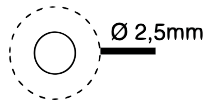
\includegraphics[scale=1.1]{3X.png} & Protégé contre les corps solides $\diameter \geq \SI{2,5}{\milli\meter}$  	& C	& 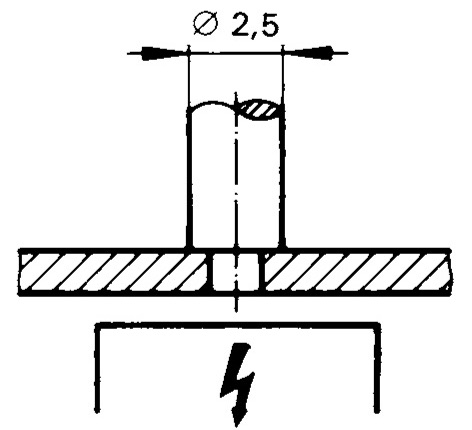
\includegraphics[width=2cm]{C.png}	&	L'introduction d'un outil ne permet pas de toucher les parties dangereuses. & 3 & 	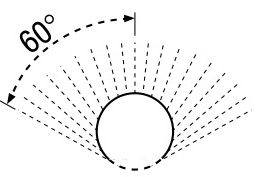
\includegraphics[scale=1.1]{X3.png}	&	Protégé contre l'eau de pluie jusqu'à 60° de la verticale \\
4 		& 	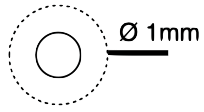
\includegraphics[scale=1.1]{4X.png} & Protégé contre les corps solides $\diameter \geq \SI{1}{\milli\meter}$  	& D	& 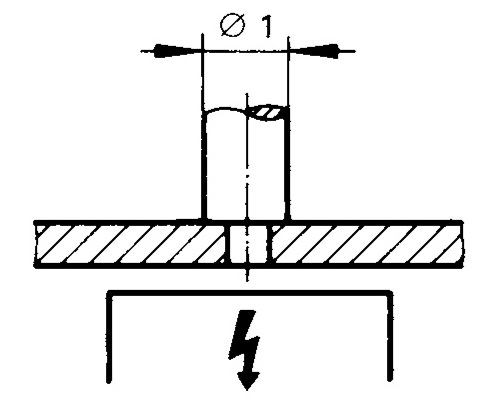
\includegraphics[width=2cm]{D.png}	&	L'introduction d'un outil fin ne permet pas de toucher les parties dangereuses. & 4 & 	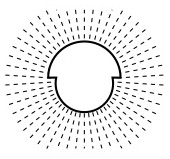
\includegraphics[scale=1.1]{X4.png}	&	Protégé contre les projections d'eau dans toutes les directions \\
5 		& 	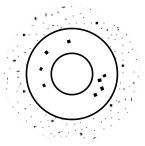
\includegraphics[scale=1.1]{5X.png} & Protégé contre la poussière (pas de dépot nuisible)  	& 	& & & 5 & 	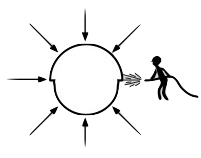
\includegraphics[scale=1.1]{X5.png}	&	Protégé contre les jets d'eau dans toutes les directions à la lance \\
6 		& 	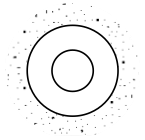
\includegraphics[scale=1.1]{6X.png} & Totalement protégé contre la poussière 	& 	& & & 6 & 	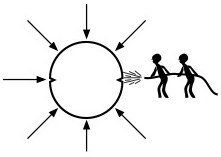
\includegraphics[scale=1.1]{X6.png}	&	Protégé contre les projections d'eau assimilables aux paquets de mer \\
 		&  & 	& 	& & & 7 & 	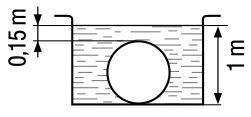
\includegraphics[scale=1.1]{X7.png}	&	Protégé contre les effets d'une immersion temporaire dans l'eau \\
		&  & 	& 	& & & 8 & 	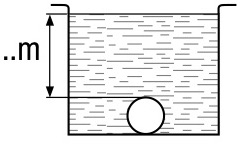
\includegraphics[scale=1.1]{X8.png}	&	Protégé contre les effets d'une immersion prolongée dans l'eau dans des conditions spécifiées \\
		&  & 	& 	& & & 9\tnote{1} & 	&	Protégé contre les jets d'eau haute pression et haute température mais pas nécessairement submersible \\
\end{xltabular}	


%\end{document}

